% 98-05(인쇄 98쪽) — 연속확률변수 X 의 확률밀도함수 y=f(x) 의 그래프(0 에서 k, 1 에서 3k 로 올랐다가 3 에서 0 으로 내려오는 꺾은선).
% 스캔 그래프가 흐려 TikZ 로 다시 그림. 라벨(3k · k · O · 1 · 3 · y=f(x))과 점선은 원문에 있는 것 그대로이고, 구하는 확률은 적지 않는다.
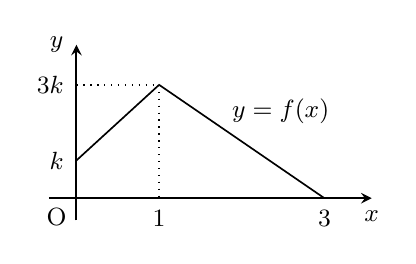
\begin{tikzpicture}[line width=0.5pt, font=\small]
  \draw[->, >=stealth, line width=0.7pt] (-0.35,0) -- (3.75,0) node[below=1pt] {$x$};
  \draw[->, >=stealth, line width=0.7pt] (0,-0.28) -- (0,1.95) node[left=1pt] {$y$};
  \node[below left=0pt] at (0,0) {O};
  \draw[line width=0.6pt] (0,0.48) -- (1.05,1.44) -- (3.15,0);
  \draw[dotted, line width=0.5pt] (0,1.44) -- (1.05,1.44);
  \draw[dotted, line width=0.5pt] (1.05,1.44) -- (1.05,0);
  \node[left=1pt] at (0,1.44) {$3k$};
  \node[left=1pt] at (0,0.48) {$k$};
  \node[below=1pt] at (1.05,0) {$1$};
  \node[below=1pt] at (3.15,0) {$3$};
  \node[above right=0pt] at (1.85,0.82) {$y=f(x)$};
\end{tikzpicture}
